\chapter{\centering\normalfont{ПРАКТИЧЕСКАЯ ЧАСТЬ}}
\label{cha:ch_2}

\section{Проектирование архитектуры}
% Какая задача поставлена
На основе данной задачи выделяются следующие подзадачи, которые необходимо
выполнить, для успешной реализации инфраструктуры:
\begin{enumerate}[label=\arabic*.]
    \item Описать возможные процессы взаимодействия между компонентами системы.
        Удобно произвести описание с помощью UML диаграммы;
    \item Смоделировать архитектуру приложения: какие компоненты будут
        взаимодействовать друг с другом;
    \item Далее равнозначные задачи, которые не обязательно выполнять
        последовательно: написать файлы запуска и написать кодовую базу для
        запуска каждой из компоненты системы.
\end{enumerate}

Далее рассмотрим каждый из пунктов подробнее, опишем способ реализации,
возникшие проблемы и пути решения.

\section{UML диаграмма}
Для наглядной демонстрации ожидаемого поведения удобно использовать подвид UML диаграмм -- диаграмму активностей.
\begin{figure}[H]
    \centering
    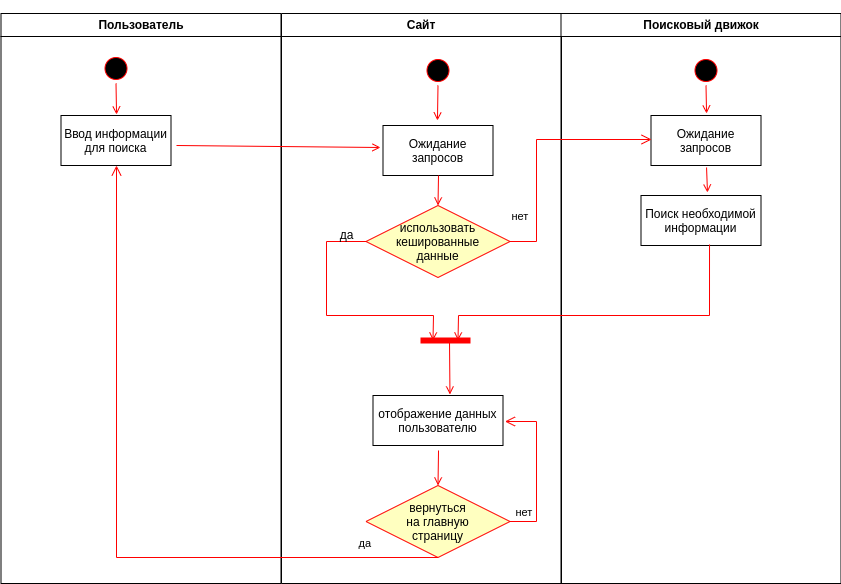
\includegraphics[scale=0.55]{inc/img/activity_diagram.png}
    \caption{Диаграмма активностей для проекта}
\end{figure}

С помощью данной диаграммы можно донести общую концепцию инфраструктуры. Также
на ее основании можно выбрать необходимые для реализации компоненты. Диаграмма
не является точным техническим заданием, а лишь выполняет демонстративную роль.

\section{Архитектура приложения}
После составления UML диаграммы можно определить свойства компонентов и
произвести их выбор.

Для наглядности составим архитектуру всего приложения.
\begin{figure}[H]
    \centering
    
\includegraphics[scale=0.70]{inc/img/structure.png}
    \caption{Архитектура приложения}
\end{figure}

В качестве web-сервера выбран Nginx с его "event based" моделью обработки
входящих соединений, которая обеспечивает быстродействие.

Web-фреймворком выступает Flask, который достаточно легковесный и позволяет
разработчику иметь больше контроля над проектом. Для того, чтобы использовать
Flask вместе с Nginx используется uwsgi.

% TODO: можно еще много чего написать про scrapy и scrapyd: что конкретно
% делают, что конкретно упрощают
Scrapy помогает разработчику извлечь необходимые данные с web-сайтов. Данный
фреймворк написан на Python и имеет открытый исходный код. Содержит в себе
большое количество настроек и достаточно масштабируем "из коробки". В
совокупности со scrapyd позволяет распологать инфраструктуру по поиску на
вычислительных серверах, а также использовать API для просмотра данных.

Для обеспечения доставки сообщений используется kafka (и его модель
Publish-Subscribe). Данный брокер сообщений снимает с приложений нагрузку
связанную с маршрутизацией и отправкой сообщений. Для оркестрации кластеров
kafka используется zookeeper.

В качестве СУБД выбран elasticsearch, т.к. им удобно пользоваться через API
запросы передавая json структуры. Можно создать несколько реплик обеспечив
отказоустойчивость системы. Где каждый узел кластера действует как координатор
для делегирования операций правильному сегменту с автоматической
перебалансировкой и маршрутизацией. Сама СУБД является документоориентированной
что избавляет разработчика от составления схем хранения, хотя для
оптимизированной работы нужно индексировать документы (без схем происходит
автоматически). При продвинутом использовании можно подключить остальные
компоненты системы, например Logstash для работы с логами.

\section{Разработка практических решений}
Спроектировав основную архитектуру и используемые модули можно приступать к
реализации конкретных компонентов.

\subsection{Scrapy}
Используя фреймворк Scrapy мы пишем абстрактные классы, называемые web-пауками,
каждый из которых можно настроить. В нем мы пишем логику перехода по ссылкам,
как с ними работать, и какие данные нужно достать со страницы.

Для начала объявляем класс "паука" в папке \verb|spiders| и задаем ему
настройки, относящиеся ко всем паукам как к единому целому:
\begin{itemize}
    \item \verb|name| -- по какому имени можно обращаться к web-паукам как к группе;
    \item \verb|custom_settings| -- общие настройки для web-пауков
\end{itemize}

\begin{verbatim}
class GithubSpider(scrapy.Spider):
    name = "github"
    custom_settings = {
        "lang_mapping": {
            "python": "Python",
        },
    }
\end{verbatim}

Настройки также можно расположить в файле \verb|settings.py|, но было решено
объявить их поближе к самому коду для легкости поиска.

Далее объявляем каким образом будут инициализироваться объекты класса. От имени
и количества входных параметров будет зависить то, какие аргументы будет
принимать консольный интерфейс Scrapy. При инициализации необходимо чтобы каждый
конкретный объект класса имел переменную \verb|start_urls| с которой он начинает
свой путь. Составляем эту переменную, используя функцию \verb|urlencode| вместе
со словарем. Крайне рекомендуется использовать специальные функции для работы с
URL, особенно если составляешь его из входных данных, т.к. должна присутствовать
функциональность экранирования специальных символов. Также проверяем
инициализированны ли входные параметры, и, если нет, то возвращаем текстовое
описание ошибки.
\begin{verbatim}
def __init__(self, topic=None, language=None, *args, **kwargs):
    super(GithubSpider, self).__init__(*args, **kwargs)

    assert topic is not None, "you should provide topic variable via cmd"
    self.topic = topic

    params = { "q": topic, }
    if language is not None:
        params.update({"l": self.custom_settings["lang_mapping"][language]})
    self.start_urls = [f"https://github.com/search?"+urlencode(params)]
\end{verbatim}

% TODO: сделать сноску с примером разбора xpath селектора
% TODO: написать про функции response.follow и response.follow_all
Пишем функцию, которая будет отвечать за переход по страницам поиска (по
страницам пагинации). В ее обязанности входит по каждому найденному репозиторию
вызвать соответствующий обработчик конкретной страницы и перейти на следующие
страницы. Для поиска ссылок для перехода (в более общей задаче -- для поиска
конкретного html элемента) применяется селекторы xpath, которые помогают
разработчику указать по каким правилам должен искаться конкретный элемент. В
данном блоке кода (и во всех функциях парсера) используется ключевое слово
\verb|yield|, которое позволяет вернуть результат вызывающей функции и
продолжить выполнение. В самом конце вызываем для всех найденных ссылок на
репозитории вызываем соответствующий обработчик.
\begin{verbatim}
def parse(self, response):
    # если есть следующая страница, запускаемся на следующей
    next_page = response.xpath('//a[@class="next_page"]/@href').get()
    if next_page is not None:
        # response.follow нативно поддерживает переход по относительным url
        yield response.follow(next_page, callback=self.parse)

    # находим репозитории на текущей странице
    repos_selector = response.xpath('//li[contains(@class, "repo-list-item")]'
                                    '//div[contains(@class, "text-normal")]'
                                    '/a')
    yield from response.follow_all(repos_selector, self.parse_repo)
\end{verbatim}

Далее нужно запарсить каждый отдельный репозиторий. Для этого реализиуем
функцию, которая будет по селекторам xpath находить нужные элементы, например,
язык программирования, популярность. Также в этом блоке кода используется
объявленные раньше общие настройки -- какой язык программирования встречается на
гитхаб, и к какому виду его нужно нормализовать (например c++ может писаться как
c++ или как cpp). В конце возвращаем словарь из данных, которые получили с
обработанной страницы.
\begin{verbatim}
def parse_repo(self, response):
    ### язык кода
    ### берем первый из списка, на проценты не смотрим
    language = response.xpath(
        '//h2[text() = "Languages"]/parent::div/ul/li/a/span/text()').get()
    # если существует конверсия в мой внутренний тип языка, то используем
    # его
    for key, val in self.custom_settings["lang_mapping"].items():
        if language == val:
            language = key
            break

    ### about
    ### у каждого репо есть короткое описание о чем он
    about = response.xpath(
        '//h2[text() = "About"]/parent::div/p/text()').get()

    ### популярность (валидна для гитхаба)
    ### (при выводе для каждого сайта надо нормализовать)
    popularity = response.xpath(
        '//span[contains(@class, "social-count")]/text()').get()

    # change how yield works
    yield {'repo_url': response.url,
            'language': language,
            'about': about,
            'popularity': popularity}
\end{verbatim}

% TODO: подробнее описать что это
Для того чтобы с возвращаемым словарем можно было работать, нужно объявить Data
Class в файле items.py.
\begin{verbatim}
import scrapy

class AlgoSearchItem(scrapy.Item):
    repo_url = scrapy.Field()
    language = scrapy.Field()
    about = scrapy.Field()
    popularity = scrapy.Field()
\end{verbatim}

Чтобы web-пауки могли пересылать свои куда либо еще (кроме базово настроенного
json файла) для начала надо модифицировать файл \verb|pipelines.py|. Пишем
инициализацию начальных переменных из файла настроек. Из него должны читаться
местоположение сервера, на котором находится брокер kafka и сам топик, куда мы
должны писать сообщения
\begin{verbatim}
class AlgoSearchPipeline:
    def __init__(self, kafka_bootstrap_server, kafka_topic):
        self.kafka_bootstrap_server = kafka_bootstrap_server
        self.kafka_topic = kafka_topic

    @classmethod
    def from_crawler(cls, crawler):
        return cls(
            kafka_bootstrap_server=crawler.settings.get('KAFKA_BOOTSTRAP_SERVER'),
            kafka_topic=crawler.settings.get('KAFKA_TOPIC')
        )
\end{verbatim}

Пишем функцию, которая запускается вместе с web-пауками. В ней создаем объект
класса KafkaProducer, который позволяет инкапсулировать в себя всю логику
сериализации сообщений.
\begin{verbatim}
def open_spider(self, spider):
    self.producer = KafkaProducer(
        bootstrap_servers=[self.kafka_bootstrap_server],
        value_serializer=lambda val: json.dumps(val,ensure_ascii=False).encode('utf-8'))
\end{verbatim}

Добавляем логику собственно отправки сообщения. В данной блоке кода мы вместе с
данными которые получаем от паука, добавляем более глобальные данные: имя паука,
адресса с которых он начал и ключевой запрос, по которому он искал. Вызывая
\verb|producer.send| мы запускаем ту инкапсулированную логику сериализации и
дальнейшую работу по маршрутизации и работе с доставкой оставляем на kafka.
\begin{verbatim}
def process_item(self, item, spider):
    # check if it has some forbidden keywords
    payload = dict(item)
    payload.update({"spider_name": spider.name,
                    "start_urls": spider.start_urls,
                    "topic": spider.topic})
    self.producer.send(self.kafka_topic, value=payload)
    return item
\end{verbatim}

% TODO: подробнее написать про логику вызовов pipeline
% TODO: сделать сноску про то, как docker разрешает сетевые вызовы, например kafka:29092
Модифицируем файл \verb|settings.py|, чтобы добавить туда необходиммые параметры
для корректной работы.
\begin{itemize}
    \item \verb|DOWNLOAD_DELAY| -- количество секунд между последовательным загрузками с сайта;
    \item \verb|CONCURRENT_REQUESTS_PER_DOMAIN| -- количество параллельных
        запросов к одному и тому же домену;
    \item \verb|ITEM_PIPELINES| -- какой pipeline использовавть вместе с пауком
        (и соотстветсвующий приоритет).
    \item \verb|KAFKA_BOOTSTRAP_SERVER|, \verb|KAFKA_TOPIC| -- на какого брокера
        kafka и в какой топик писать сообщения.
\end{itemize}
\begin{verbatim}
DOWNLOAD_DELAY = 2
CONCURRENT_REQUESTS_PER_DOMAIN = 1
ITEM_PIPELINES = {
    'algo_search.pipelines.AlgoSearchPipeline': 300,
}
KAFKA_BOOTSTRAP_SERVER = "kafka:29092"
KAFKA_TOPIC = "algorithms-events"
\end{verbatim}

% TODO: сделать сноску на разницу json и jl
Для вызова парсера на стадии разработки, нам понадобится команда для запуска и
несколько основных аргументов запуска:
\begin{itemize}
    \item \verb|scrapy crawl github| -- запускает пауков;
    \item \verb|-O file.json| -- пишет выходные данные в файл \verb|file.json|;
    \item \verb|-o file.jl| -- пишет выходные данные в файл \verb|file.jl|;
    \item \verb|-a topic=ukkonen| -- передает аргумент на вход паукам.
\end{itemize}

% TODO: проверка работы

\subsection{Zookeeper}
Перед разворачиванием kafka нужно сначала запусть zookeeper. Последний используется для синхронизации сервисов.

В данном случае картинкой контейнера будет служить
\verb|confluentinc/cp-zookeeper:latest|. Данная картинка позволяет заменить
конфигурационный файл набором переменных окружения, которые следуют специальным
правилам именования.

Обязательным параметром при развертывании является \verb|ZOOKEEPER_CLIENT_PORT|
-- порт, который прослушивается на входящие соединения. Также задаем параметр
\verb|ZOOKEEPER_TICK_TIME| -- является базовой единицей измерения времени и
регулирует таймауты.

% TODO: сделать сноску почему для zookeeper важно хранить логи
Далее, для того чтобы данные не стирались от запуска к запуску (например при
перезагрузке), необходимо добавить ссылки на хранилище на хосте docker. Создаем
папки \verb|vol1/zk-data| и \verb|vol2/zk-txn-logs| для хранения данных
\verb|zookeeper|. Соотношение папок хоста к клиенту будет таким:
\begin{itemize}
    \item \verb|vol1/zk-data| -- \verb|/var/lib/zookeeper/data|
    \item \verb|vol2/zk-txn-logs| -- \verb|/var/lib/zookeeper/log|
\end{itemize}

Также необходимо переопределить порты которые связаны с клиентов, чтобы не было
случайных коллизий. Будем использовать порт на хосте 22181 и с него будут
перенаправляться запросы на порт 2181 в \verb|zookeeper|.

Даем запускаемому контейнеру имя \verb|zookeeper| и составляем часть файла
развертывания \verb|docker-compose.yml|
\begin{verbatim}
zookeeper:
  image: confluentinc/cp-zookeeper:latest
  container_name: zookeeper
  environment:
      ZOOKEEPER_CLIENT_PORT: 2181
      ZOOKEEPER_TICK_TIME: 2000
  volumes:
      - ./vol1/zk-data:/var/lib/zookeeper/data
      - ./vol2/zk-txn-logs:/var/lib/zookeeper/log
  ports:
      - 22181:2181
\end{verbatim}

% TODO: проверка работы

\subsection{Kafka}
Далее развернем менеджер сообщений. Он возмет на себя роль посредника между
приложением, которое генерирует данные и приложением, которое эти данные должно
получить.

Для начала необходимо определиться с картинкой контейнера, которую хотим
запустить. В нашем случае это будет \verb|confluentinc/cp-kafka:latest|.

% TODO: о том, какие бывают протоколы безопасности подключений и как они
% работают
К обязательным параметрам при развертывании относятся:
\begin{itemize}
    \item \verb|KAFKA_ZOOKEEPER_CONNECT| -- как подключиться к \verb|zookeeper|.
        Задаем значение \verb|zookeeper:2181|;
    \item \verb|KAFKA_ADVERTISED_LISTENERS| -- описывается имя хоста и как оно
        может быть достигнуто клиентами. Значение публикуется в
        \verb|zookeeper|. Задаем значение
        \verb|PLAINTEXT://kafka:9092,PLAINTEXT_HOST://kafka:29092|. Брокер
        возвращает данное значение клиенту для того, чтобы показать куда
        отправлять данные;
    \item \verb|KAFKA_OFFSETS_TOPIC_REPLICATION_FACTOR| -- количество
        дублирований, которые kafka создает на узлах. Должно быть меньше или
        равно количеству запущенных узлов. В нашемм случае обязательно задать
        единицу, так как базовое значение этого параметра равно трем;
    \item \verb|KAFKA_LISTENER_SECURITY_PROTOCOL_MAP| -- задаем протокол
        безопасности для подключений к указанным хостам. В нашем случае
        \verb|PLAINTEXT:PLAINTEXT,PLAINTEXT_HOST:PLAINTEXT|.
\end{itemize}

Для того, чтобы уникально идентифицировать созданный узел, задаем ему
\verb|broker.id| равным 1. Порты на хосте docker и в контейнере kafka оставляем
одинаковыми (т.к. мы уже опредилили к какому порту подключаться при конфигурации
kafka выше) -- 29092 к 29092.

Далее нам потребуется сохранять данные от запуска к запуску. Поэтому создаем
папки \verb|vol3/kafka-data| на хосте и указываем с какой папкой последняя из
них будет соотносится -- \verb|/var/lib/kafka/data|.

Совмещая все вышесказанное про kafka в структурированный docker-compose формат и
получаем блок конфигурационного файла, который отвечает за развертывание kafka.
\begin{verbatim}
kafka:
  image: confluentinc/cp-kafka:latest
  container_name: kafka
  depends_on: # запускаемся после zookeeper'а
    - zookeeper
  ports:
    - 29092:29092
  volumes:
    - ./vol3/kafka-data:/var/lib/kafka/data
  environment:
    KAFKA_BROKER_ID: 1
    KAFKA_ZOOKEEPER_CONNECT: zookeeper:2181
    KAFKA_ADVERTISED_LISTENERS: PLAINTEXT://kafka:9092,PLAINTEXT_HOST://kafka:29092
    KAFKA_LISTENER_SECURITY_PROTOCOL_MAP: PLAINTEXT:PLAINTEXT,PLAINTEXT_HOST:PLAINTEXT
    KAFKA_OFFSETS_TOPIC_REPLICATION_FACTOR: 1
\end{verbatim}

Заметим, что сервис kafka должен запускаться строго после того, как запуститься
менеджер сервисов zookeeper. По этой причине выше добавлена опция
\verb|depends_on: - zookeeper|

% TODO: проверка работы

\subsection{Elastic Search}
Elasticsearch будет хранить и возвращать данные на постоянной основе. Данные
принимаются согласно архитектуре -- от kafka, которая, в свою очередь принимает
их от scrapy.

Выбираем картинку конейнера. В нашем случае это \verb|elasticsearch:6.5.0|. Тут
пришлось потратить много времени на выбор картинки, так как из-за запретов,
некоторые картинки невозможно было скачать. Сразу же выбираем имя для
работающего контейнера -- \verb|es1|

Для того, чтобы данные оставались после перезагрузки контейнера, будем
записывать некоторые папки на хост docker. Поэтому создаем папку \verb|es-data|
на хосте и ставим ей в соответствие папку \verb|/usr/share/elasticsearch/data| в
контейнере. Эти две папки имеют прямую синхронизацию, и, соответсвенно, при
перезагрузке данные остануться.

Далее задаем несколько параметров работы elasticsearch (большое количество
настроек может быть обновленно во время работы с помощью специального
интерфейса):
\begin{itemize}
    \item \verb|http.host: 0.0.0.0| -- адресс узла для входящих HTTP соединений;
    \item \verb|transport.host: 0.0.0.0| -- адресс узла для коммуникации между узлами;
    \item \verb|discovery.type: "single-node"| -- необходимый параметр для
        запуска одного узла (данный узел объявляет себя мастер узлом и не
        присоединяется к кластеру);
    \item \verb|xpack.security.enabled: "false"| -- выключаем работу модуля
        \verb|xpack.security|. Данный модуль можно использовать для настройки
        анонимного доступа, аутентификации сообщений, уровней доступа к
        документам и их полям и т.д.;
    \item \verb|ES_JAVA_OPTS: "-Xms1g -Xmx1g"|, \verb|ES_JAVA_OPTIONS: "-Xms1g
        -Xmx1g"| -- задаем начальный и максимальный размеры кучи для
        elasticsearch;
\end{itemize}

Устанавливаем соответствие портов на хосте docker и контейнере:
\verb|9200:9200|, \verb|9300:9300|.

Получаем готовый файл конфигурации для запуска сервиса elasticsearch:
\begin{verbatim}
elasticsearch:
  image: elasticsearch:6.5.0
  container_name: es1
  ports:
    - 9200:9200
    - 9300:9300
  volumes:
    - ./es-data:/usr/share/elasticsearch/data
  environment:
    http.host: 0.0.0.0
    transport.host: 0.0.0.0
    discovery.type: "single-node"
    xpack.security.enabled: "false"
    ES_JAVA_OPTS: "-Xms1g -Xmx1g"
    ES_JAVA_OPTIONS: "-Xms1g -Xmx1g"
\end{verbatim}

% TODO: проверка работы

\subsection{Kafka Connect}
Далее нужно настроить такое поведение, при котором kafka поступающие в топик
сообщения будет перенаправлять в соответствующий индекс в elasticsearch. Для
задач такого рода был создан продукт kafka connect.

Выбираем картинку того же разработчика, от которого мы брали kafka и zookeeper
-- \verb|confluentinc/cp-kafka-connect:3.3.0|.

Для того, чтобы созданные коннекторы оставались от запуска к запуску,
настраиваем синхронизацию папки \verb|/connect-plugins| с папкой
\verb|connect-plugins| на хосте docker.

Настраиваем установку с помощью параметров:
\begin{itemize}
    \item \verb|CONNECT_BOOTSTRAP_SERVERS: kafka:9092| -- где развернут брокер kafka;
    \item \verb|CONNECT_ZOOKEEPER_CONNECT: zookeeper:2181| -- где развернут zookeeper;
    \item \verb|CONNECT_REST_PORT: 8083| -- порт для входящих соединений API;
    \item \verb|CONNECT_PLUGIN_PATH: /connect-plugins| -- где будут
        распологаться сами коннекторы; 
    \item \verb|CONNECT_REST_ADVERTISED_HOST_NAME: "connect"| -- по какому хосту
        клиентам можно отправлять сообщения;
    \item \verb|CONNECT_GROUP_ID: "connect"| -- может быть любым, используется
        для того, чтобы узлы определяли к какому кластеру они принадлежат;
    \item \verb|CONNECT_CONFIG_STORAGE_TOPIC|,
        \verb|CONNECT_OFFSET_STORAGE_TOPIC|, \verb|CONNECT_STATUS_STORAGE_TOPIC|
        -- имена топиков, в которых сохранять служебную информацию;
    \item \verb|CONNECT_REPLICATION_FACTOR|,
        \verb|CONNECT_CONFIG_STORAGE_REPLICATION_FACTOR|,
        \verb|CONNECT_OFFSET_STORAGE_REPLICATION_FACTOR|,
        \verb|CONNECT_STATUS_STORAGE_REPLICATION_FACTOR| -- отвечают за
        дублированние данных в кластере. Так как узел всего один, то в этих
        параметрах ставим единицу;
    \item \verb|CONNECT_KEY_CONVERTER|, \verb|CONNECT_VALUE_CONVERTER|,
        \verb|CONNECT_INTERNAL_KEY_CONVERTER|,
        \verb|CONNECT_INTERNAL_VALUE_CONVERTER| -- настройка для сериализации и
        десериализации ключей и значений;
    \item \verb|CONNECT_VALUE_CONVERTER_SCHEMAS_ENABLE: "false"| -- так как json
        не включает в себя схему и не используется регистратор схем, то ставим
        значение \verb|false|.
\end{itemize}

Получаем сегмент конфигурационного файла для развертывания сервиса kafka
connect:
\begin{verbatim}
connect:
  build: ./kafka-connect
  container_name: kafka_connect
  ports:
    - 8083:8083
  depends_on:
    - zookeeper
    - kafka
  volumes:
    - $PWD/connect-plugins:/connect-plugins
  environment:
    CONNECT_BOOTSTRAP_SERVERS: kafka:9092
    CONNECT_REST_PORT: 8083
    CONNECT_GROUP_ID: "connect"
    CONNECT_CONFIG_STORAGE_TOPIC: connect-config
    CONNECT_OFFSET_STORAGE_TOPIC: connect-offsets
    CONNECT_STATUS_STORAGE_TOPIC: connect-status
    CONNECT_REPLICATION_FACTOR: 1
    CONNECT_CONFIG_STORAGE_REPLICATION_FACTOR: 1
    CONNECT_OFFSET_STORAGE_REPLICATION_FACTOR: 1
    CONNECT_STATUS_STORAGE_REPLICATION_FACTOR: 1
    CONNECT_KEY_CONVERTER: "org.apache.kafka.connect.storage.StringConverter"
    CONNECT_VALUE_CONVERTER: "org.apache.kafka.connect.json.JsonConverter"
    CONNECT_VALUE_CONVERTER_SCHEMAS_ENABLE: "false"
    CONNECT_INTERNAL_KEY_CONVERTER: "org.apache.kafka.connect.json.JsonConverter"
    CONNECT_INTERNAL_VALUE_CONVERTER: "org.apache.kafka.connect.json.JsonConverter"
    CONNECT_REST_ADVERTISED_HOST_NAME: "connect"
    CONNECT_ZOOKEEPER_CONNECT: zookeeper:2181
    CONNECT_PLUGIN_PATH: /connect-plugins
\end{verbatim}

% TODO: проверка работы

\subsection{Flask}
Далее реализуем часть, которая будет принимать и обрабатывать запросы
пользователя, а затем, возвращать отображаемую страницу. Для этой подзадачи
будем использовать web-фреймворк Flask. В нем нет специальной структуры
директориев, правил работы с базами данных или файлами настроек, поэтому будем
реализовывать эту часть сами.

Начнем с выбора картинки контейнера, в нашем случае это будет
\verb|tiangolo/uwsgi-nginx-flask:python3.8-alpine|. Как видно по названию,
картинка уже включает в себя установленные \verb|nginx|, \verb|uwsgi| и
\verb|flask|. Данные пакеты были поставлены на достаточно маленький дистрибутив
\verb|Alpine Linux|, который не займет много времени для загрузки.

Для начальной конфигурации контейнера, необходимо сделать несколько шагов
(каждый из которых, создает новый слой картинки):
\begin{enumerate}[label=\arabic*.]
    \item Установить пакеты \verb|bash|, \verb|vim|;
    \item Задать в переменных окружения значения для работы со статичными
        данными (css, media) для Nginx: \verb|STATIC_URL| (по какому адрессу
        получаются статичные данные), \verb|STATIC_PATH| (по какому пути в
        системе эти данные достаются);
    \item Задать переменные окружения для среды разработки: \verb|FLASK_ENV|, \verb|FLASK_DEBUG|;
    \item Установить зависимости;
\end{enumerate}

Составляем из всего вышесказанного \verb|Dockerfile|, получим:
\begin{verbatim}
FROM tiangolo/uwsgi-nginx-flask:python3.8-alpine
RUN apk --update add bash vim
ENV STATIC_URL /static
ENV STATIC_PATH /app/app/static
ENV FLASK_ENV development
ENV FLASK_DEBUG 1
COPY ./requirements.txt /var/www/requirements.txt
RUN pip install --no-cache-dir --upgrade -r /var/www/requirements.txt
\end{verbatim}


Далее определим параметры запуска самого контейнера:
\begin{itemize}
    \item Именем контейнера будет являться \verb|flask-server|;
    \item Директория, в которой находится \verb|Dockerfile| -- \verb|flask_server|;
    \item Соответствие портов на хосте docker и в самом контейнере -- \verb|56733:80|;
    \item Директория с кодом должна распологаться в контейнере в папке \verb|app| (для запуска).
\end{itemize}

Получим сегмент конфигурационного файла для развертывания сервера:
\begin{verbatim}
flask-server:
  container_name: flask-server
  build:
    context: ./flask_server
    dockerfile: ./Dockerfile
  ports:
    - 56733:80
  volumes:
    - ./flask_server:/app
\end{verbatim}

Для того, чтобы Flask приложение запускалось, создадим файл \verb|uwsgi.ini| со следующим содержанием:
\begin{verbatim}
[uwsgi]
module = main
callable = app
master = true
touch-reload = /app/uwsgi.ini
\end{verbatim}

Таким образом мы сообщаем uwsgi (он, в свою очередь будет общаться с Nginx), что
код запуска приложения будет находится в файле \verb|main.py|, а вызываемая
функция будет называться \verb|app|. Также данный объект будет является мастер
узлом и для того, чтобы его перезагрузить, надо вызвать команду \verb|touch
/app/uwsgi.ini|.

Файл \verb|main.py| будет загружать решение из поддиректории: \verb|from app
import app|.

Далее, в поддиректории \verb|app| создаем файл \verb|__init__.py| (который
отвечает за то, как эта директория импортируется). В нем мы указываем что будем
работать с модулем Flask. Затем в этом же файле мы создаем инициализируем
веб-сервер (начинаем с ним работу) и импортируем функции из файла
\verb|views.py|.
\begin{verbatim}
from flask import Flask
app = Flask(__name__)
from app import views
\end{verbatim}

Файл \verb|views.py| будет содержать генерации и отображения отображения страниц
пользователю.

% TODO: не знаю, нужно ли указывать тут сами html страницы, т.к. много текста
% выйдет
Первым делом необходимо добавить домашнюю страницу:
\begin{verbatim}
@app.route('/')
def home():
    return render_template('home.html')
\end{verbatim}

\verb|render_template| позволяет передавать в шаблонизатор \verb|Jinja|
параметры для динамической генерации html страниц.

% TODO: сделать сноску что делают декораторы в python
В декораторе \verb|app.route| необходимо указать уникальный путь, за который
будет отвечать данная функция. Также там можно указать за какие методы запросов
данная функция будет отвечать (GET, POST, PATCH и так далее)

На главной странице присутствует ссылка по переходу на страницу по поиску
алгоритмов. Напишем для этой страницы обработчик. Указываем относительный путь,
который будет обрабатываться функцией и объявляем ее:
\begin{verbatim}
@app.route('/search_by_name', methods=["GET", "POST"])
def search_by_name():
\end{verbatim}

Затем, если был использован GET запрос, то из адрессной строки можно выбрать
параметры запроса. Этим и займемся. 
\begin{verbatim}
search_object = request.args.get("search_object")
search_lang = request.args.get("search_lang")
\end{verbatim}

Если хотя бы один из параметров пустой, то возвращаем поисковую страницу, на
которой эти параметры можно заполнить.
\begin{verbatim}
if search_object is None and search_lang is None:
    return render_template('search_by_name.html')
\end{verbatim}

Если запрос не подходит под это условие, значит: либо мы сами сконструировали
URL адресс и хотим сделать запрос, либо мы уже были на этой странице и уже
заполнили все необходимые параметры. В любом из этих случаев нам необходимо
произвести запросы к базе данных и вернуть пользователю информацию.

Для начала составляем запрос для поиска сохраненных репозиториев в elastic search:
\begin{verbatim}
data_for_cache_hits = {
    "query": {
        "bool": {
            "must": [
                {"match": {"topic": search_object}},
                {"match": {"language": search_lang}},
            ]
        }
    },
}
\end{verbatim}

Затем отправляем этот запрос на сервер с elasticsearch:
\begin{verbatim}
s = requests.Session()
retries = Retry(total=5,
                backoff_factor=0.1,
                status_forcelist=[500,502,503,504])
s.mount('http://', HTTPAdapter(max_retries=retries))
params = {'size': 10000, }
es_hits_resp = s.get('http://elasticsearch:9200/algorithms-events/_search',
                     params=params,
                     json=data_for_cache_hits,
                     verify=False)
es_hits_data = es_hits_resp.json()
\end{verbatim}

Обрабатываем полученные данные и возвращаем страницу пользователю:
\begin{verbatim}
hits_qty = es_hits_data['hits']['total']
hits_data = [hit['_source'] for hit in es_hits_data['hits']['hits']]

for hit in hits_data:
    hit['popularity'] = int(hit['popularity'])
return render_template('search_by_name.html',
                        search_object=search_object,
                        search_lang=search_lang,
                        hits_data=hits_data)
\end{verbatim}

Следует дополнить данный функционал запросами по обновлению данных в
elasticsearch и по очистке этих данных.
\begin{verbatim}
@app.route('/update_es', methods=["GET"])
def update_es():
    topic = request.args.get("topic")
    language = request.args.get("language")
    params = {
        "project":  "algo_search",
        "spider":   "github",
        "topic":    topic,
        "language": language,
    }
    with requests.post("http://scrapyd:6800/schedule.json", params=params) as resp:
        print(resp.status_code)
        print(resp.json())

    return redirect(url_for("search_by_name",
                            search_object=topic,
                            search_lang=language))

@app.route('/clear_es', methods=["GET"])
def clear_es():
    topic = request.args.get("topic")
    language = request.args.get("language")

    data = {"query": {"match_all": {}}}
    with requests.post("http://elasticsearch:9200/algorithms-events/_delete_by_query",
                       json=data) as resp:
        print(resp.status_code)
        print(resp.json())

    return redirect(url_for("search_by_name",
                            search_object=topic,
                            search_lang=language))
\end{verbatim}

Конечная структура директории веб-сервиса:
\begin{verbatim}
.
├── app
│   ├── __init__.py
│   ├── static
│   │   └── styles
│   │       └── main.css
│   ├── templates
│   │   ├── home.html
│   │   ├── layout.html
│   │   ├── search_by_name.html
│   └── views.py
├── Dockerfile
├── main.py
├── requirements.txt
└── uwsgi.ini
\end{verbatim}

% TODO: проверка работы

\subsection{Scrapyd}
Выбираем картинку \verb|vimagick/scrapyd:py3|. Далее устанавливаем зависимости
добавляя в нее новый слой. Получаем \verb|Dockerfile|:
\begin{verbatim}
FROM vimagick/scrapyd:py3
COPY requirements.pip ./
RUN pip install -r requirements.pip
\end{verbatim}

Даем запускаемому контейнеру имя \verb|scrapyd| и указываем в какой директории
находится файл для сборки. Также указываем соответствие портов на хосте и в
контейнере \verb|6800:6800|.

Для того, чтобы находящиеся там проекты Scrapy не удалялись, необходимо
настроить синхронизацию папок: создаем папку \verb|scrapyd-data| и указываем ей
в соответствие папку \verb|/var/lib/scrapyd|.

Для того, чтобы положить пауков на этот сервер, используем утилиту
\verb|scrapyd-deploy|.

Также можно зайти на адресс, по которому расположен сервер и посмотреть
информацию по находящимся там web-паукам и задачам. Например, зайдя на адресс
\verb|http://localhost:6800/listprojects.json| можно посмотреть список доступных
проектов, а сделав POST-запрос на адресс
\verb|http://localhost:6800/schedule.json| можно запустить конкретного паука.

% TODO: проверка работы
